\documentclass[../TV&MS.tex]{subfiles}
\begin{document}
    
\section{Случайные величины}

\subsection{Случайные величины: определение}

\qquad Случайные события "--- это хорошо, но события типа <<на монетке выпал герб>> плохо формализуемы, 
а мы хотим формальности и математичности. Поэтому вместо всяких событий хочется работать с числами. 
Вот этим и займемся. При рассмотрении случайных событий мы ввели вероятностное пространство, 
которое выглядит так:
$$(\Omega, \Ev, \Pro),$$

где $\Omega$ "--- множество элементарных событий, $\Ev$ "--- $\sigma$-алгебра подмножеств 
множества элементарных событий, а $\Pro$ "--- вероятность. Мы же будем рассматривать теперь тройку
$$(\Real, \Bor, \Pro),$$

где $\Real$ "--- действительная прямая, $\Bor$ "--- борелевская $\sigma$-алгебра, а $\Pro$ "--- вероятность.


Теперь формально введем понятие случайной величины (может использоваться сокращение с.в.).

\begin{Def}
Пусть $(\Omega, \Ev, \Pro)$ "--- вероятностное пространство. Тогда \mdef{случайной величиной $\xi$} 
называется функция $\xi : \Omega \to \Real$, измеримая относительно $\Ev$ и $\Bor$. 
По-другому, $\xi$ "--- случайная величина, если
$$\forall B \in \Bor \quad \xi^{-1}(B) = \lbrace \omega : \xi(\omega) \in B \rbrace \in \Ev.$$
\end{Def}

\begin{Wtf}
Таким финтом ушами мы, по сути, сопоставили каждому событию какое-то <<хорошее>> множество на 
числовой прямой, и можем рассматривать не вероятности событий, а вероятности попадания в эти 
<<хорошие>> подмножества числовой прямой.
\end{Wtf}

\subsection{Функция распределения}

Введем еще несколько <<полезных>> определений, которые в дальнейшем использоваться не будут,
но знать их не вредно.

\begin{Def}
С каждой случайной величиной свяжем два вероятностных пространства: первое --- 
$(\Omega, \Ev_\xi, \Pro)$ --- вероятностное пространство, \mdef{порожденное $\xi$}. 
Здесь $\Ev_\xi$ - наименьшая $\sigma$-алгебра, для которой выполняется свойство измеримости. 
Второе --- $(\Real, \Bor, \Pro_\xi)$, где $\Pro_\xi(B) = \Pro(\xi^{-1}(B)) \quad \forall B \in \Bor$ 
и называется \mdef{распределением вероятностей $\xi$}.
\end{Def}

Идем дальше в~сторону упрощения работы со случайностями. Вместо того чтобы рассматривать произвольные 
борелевские множества, мы будем рассматривать только множества вида $(-\infty, x)$. Действительно, 
интервал $(a, b)$ получается из~полупрямых так: $(a, b) = (-\infty, b) \setminus (-\infty, a]$.  
Таким образом, мы можем рассматривать случайные величины только на таких множествах. Здесь имеется в виду, 
что для удовлетворения определению случайной величины достаточно измеримости только на
полупрямых, что следует из следующих свойств полного прообраза: прообраз объединения есть объединение 
прообразов, прообраз пересечения есть пересечение прообразов, прообраз отрицания есть отрицание прообраза. 
Выше показано, что из полупрямых с помощью этих операций можно получить интервалы, а из интервалов и все 
$\Bor$.

Теперь несколько полезных утверждений. Пусть $\xi$ --- случайная величина. Тогда $-\xi$ также 
случайная величина, так как её прообраз от любой полупрямой является прообразом $\xi$ от 
симметричной полупрямой, то есть лежит в $\Ev$. Величина $\xi + c$ также будет случайной величиной, 
поскольку ее прообразом для любой полупрямой будет прообраз $\xi$ для полупрямой, сдвинутой на $c$, 
то есть будет лежать в $\Ev$.

\begin{St}
Пусть $\xi, \eta$ --- случайные величины. Тогда множество $\left\{\omega \colon
\xi(\omega) < \right.$ $\left. \eta(\omega)\right\}$ является событием.
\end{St}
\begin{Proof}
$\Set{\omega}{\xi(\omega) < И\eta(\omega)} = \bigcup\limits_{r \in \mathbb{Q}}
\Set{\omega}{\xi(\omega) < r, \eta(\omega) > r}$. 
Заметим, что $\Set{\omega}{\xi(\omega) < r}$ является событием. Аналогично для $\eta$. 
Выражение, написанное выше, является счетным объединением пересечений двух событий, то есть событием.
\end{Proof}

Похожими махинациями, а также с использованием этого утверждения, доказывается, что 
$\xi^2, \xi + \eta, \xi\eta$ являются случайными величинами.
Более того, если $\xi_1, \ldots, \xi_n$~---~с.в., а функция $\phi(x_1, \ldots, x_n)$ 
является непрерывной на множестве их значений, то $\phi(\xi_1, \ldots, \xi_n)$ будет случайной 
величиной. 

\begin{Def}
Рассмотрим вероятностное пространство $(\Omega, \Ev, \Pro)$ и определенную на нем 
случайную величину $\xi$. Тогда её \mdef{функцией распределения $F_\xi(x)$}
называется функция $F_\xi : \Real \to \Real$
$$F_\xi(x) = \Pro(\omega : \xi(\omega) < x) = \Pro(\xi < x)$$.
\end{Def}

Запись $\Pro(\xi < x)$ является в некотором смысле жаргонной, так как аргументов 
вероятности должно быть событие из $\Ev$. Но $\xi < x$ мы в дальнейшем будем 
отождествлять с объединением элементарных событий, образ которых меньше $x$. Из определения 
случайной величины получаем, что это объединение является событием,
поэтому применение к нему функции вероятности корректно.

Функция распределения (сокращение ф.р.) является очень полезной штукой, поскольку имеет 
достаточно простой вид и несет в себе всю информацию о распределении, то есть однозначно 
определяет $\Pro_\xi$.

Рассмотрим основные свойства функции распределения:
\begin{enumerate}
	\item $F_\xi(x) \in [0, 1]$
	\item $\lim\limits_{x \to -\infty} F_\xi(x) = 0$
	\item $\lim\limits_{x \to +\infty} F_\xi(x) = 1$
	\item $F_\xi(x)$ монотонно не убывает.
	\item $F_\xi(x)$ непрерывна слева.
\end{enumerate}

Вероятность попадания с.в. в полуинтервал $\Pro_\xi[a,b) = F_\xi(b) - F_\xi(a)$. При 
стремлении $b \to a$ получим $\Pro(\xi = a) = F_\xi(a+0) - F_\xi(a)$, то есть 
вероятность попадания в точку равна скачку функции распределения в этой точке.

\begin{Def}
Точка $x_0$ называется \mdef{точкой роста} $F_\xi(x)$, если $\forall \varepsilon > 0 \quad$
$\Pro(x_0 -~\varepsilon \le \xi < x_0 + \varepsilon) > 0$
\end{Def}

\begin{Ex}
Это очень полезный пример, который будет использоваться в матстате и который очень любят спрашивать. 
Пусть $\xi$ --- случайная величина. $\eta = F_\xi(\xi)$. Чему равна $F_\eta(x)$? По определению 
\begin{equation}\label{fXiOfXi}
F_\eta(x) = \Pro(\eta < x) = \Pro(F_\xi(\xi) < x)=\Pro(\xi < F_\xi^{-1}(x)) = F_\xi(F_\xi^{-1}(x))=x
\end{equation}
Вообще, тут было бы неплохо сказать, что $F_\xi$ непрерывна и строго монотонна, чтобы со спокойной 
совестью использовать обратную функцию. Таким образом $\eta$ имеет равномерное распределение.
\end{Ex}

\subsection{Виды распределений}

Распределения случайных величин можно разделить на $3$ типа: непрерывные, дискретные и сингулярные.

\begin{Def}
	Случайная величина $\xi$ называется \mdef{абсолютно непрерывной}, если существует интегрируемая 
	функция $p_\xi(x) \ge 0, \ x \in \Real$ такая, что функция распределения $\xi$ является почти всюду 
	(за исключением не более, чем счетного числа точек) дифференцируемой функцией и представима в виде
	$$F_\xi(x) = \int\limits_{-\infty}^x p_\xi(y)dy$$
	Отсюда следует, что функция распределения непрерывна на $\Real$. $p_\xi(x)$ называется 
	\mdef{плотностью распределения}, и почти всюду выполнено $p_\xi(x)=F_\xi'(x)$.
	Плотность, вообще говоря, определена не однозначно.
\end{Def}

\begin{Def}
	Случайная величина $\xi$ называется \mdef{дискретной}, если множество точек роста не более, 
	чем счетно, но распределение не является сингулярным, или, 
	другими словами $\exists B = \{x_1, x_2, \ldots\} \colon \Pro(\xi \in B) = 1$.
\end{Def}

\begin{Def}
	Случайная величина $\xi$  называется \mdef{сингулярной}, если $F_\xi$ непрерывна, и 
	$\exists B \in \Bor \colon \mu(B) = 0, \ \Pro(\xi \in B) = 1$, то есть множество значений 
	случайной величины имеет меру 0, но вероятность попасть в каждую точку этого множества так же нулевая.
\end{Def}

Пара слов о жизненном смысле определений: непрерывная случайная величина имеет областью значений 
континуальное множество, при этом вероятность попасть в отдельно взятую точку нулевая. Пример: 
равномерное распределение по отрезку. Плотность же отражает вероятность попасть в ту или иную область: 
интеграл по области равен этой вероятности. Дискретная случайная величина принимает конечное или счетное 
множество значений, вследствие этого имеет ступенчатую функцию распределения, например, бросок монетки 
имеет дискретное распределение. Сингулярное распределение --- это крокодил, который не встречается в жизни 
и будет рассмотрен отдельно.

\begin{St}
	Дискретная случайная величина имеет не более, чем счетное число скачков.
\end{St}
\begin{Proof}
Из свойств функции распределения следует, что дискретная величина имеет не больше 
двух скачков величины больше $\frac12$. Аналогично, скачков величины больше $\frac13$ 
не больше $3$. То есть скачков величины больше $\frac1n$ не более $n$. Для любого скачка 
можно указать $n \in \mathbb{N}$ такое, что величина, этого скачка больше $\frac1n$. 
Значит,каждому скачку можно поставить в соответствие $n$, множество которых счетно. 
При этом для каждого $n$ существует не более чем счетное число скачков, ему соответствующих 
(величины $>\frac1n$). А так как объединение не более, чем счетного числа не более, чем 
счетных множеств, не более, чем счетно, получаем требуемое. 
\end{Proof}

\begin{Ex}
Для полного счастья приведем пример сингулярной случайной величины. Пусть функция 
распределения~---~так называемая лестница Кантора (см. рисунок).
\parbox[b][3 cm][t]{20mm}{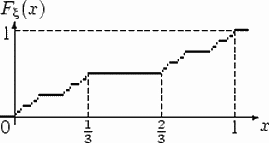
\includegraphics[height=30mm]{kantor}}
\hfill
\parbox[b][3 cm][t]{100mm}{
	Посчитаем меру множества, на котором функция константа, то есть точки этого множества не 
	будут точками роста: сначала это одна ступенька длины $1/3$, потом две длины $1/9$, и т.\,д.
}\\
	$$ \frac13 + \frac29 + \frac4{27} = \frac13 \sum\limits_{k=1}^\infty(\frac23)^{k-1} = 1.$$

	Тогда множество точек роста имеет меру $0$ в силу свойства аддитивности меры.
\end{Ex}

Вообще говоря, существуют менее изысканные примеры сингулярных распределений. Например, при 
стрельбе из лука в круглую мишень распределение будет сингулярным, если стрелок попадает только 
в точки одной прямой. В самом деле, двумерная мера прямой равна $0$, как и вероятность 
попасть в каждую отдельную точку. 

\begin{Th} [Лебега]
	Любую случайную величину можно представить в виде суммы дискретной, абсолютно непрерывной и 
	сингулярной случайной величины. То есть 
	$$ F(x) = \alpha_dF_d(x) + \alpha_cF_c(x) + \alpha_sF_s(x), 
	\quad \alpha_d + \alpha_c + \alpha_s = 1.$$
\end{Th}
\begin{Proof}
Не вошло в содержание и не вышло с публикацией. Ищите в других учебниках.
\end{Proof}

\newpage



\end{document}
